\section{Applications for Large Models}
\label{sec:applications}

In this section, we look at examples for three modeling applications. We do this for two reasons. The first reason is to discuss the actual practical relevance of large models. The second reason is to identify model usage patterns: which of the four modeling tasks (create, traverse, query, partial load) are actually used, in what frequency, and with what parameters. At the end of this section, we provide a tabular summary of our assessment.

\subsection{Software Models}
Model Driven Software Development (MDSD) is the application that modelling frameworks like EMF were actually designed for. In MDSD all artifacts including traditional software models as well as software code are understood as models~\cite{modelsAsCode}, i.e. directed labelled graphs of typed nodes with an inherent containment hierarchy. 

\tinyparagraph{Model size} Since models of software code (code models) provide the lowest level of abstraction, we assume that models of software code are the largest software models. In~\cite{modelSizes}, we give an approximation for the size of code models based on counting abstract syntax tree nodes in the Linux kernel and analyzing the Linux kernels GIT repository. We also transferred all ratios learned from the Kernel to other OS software projects and publicly reported LOC counts. The results are presented in Fig.~\ref{fig:software_model_sizes}.

\begin{figure}[b]
  \centering
  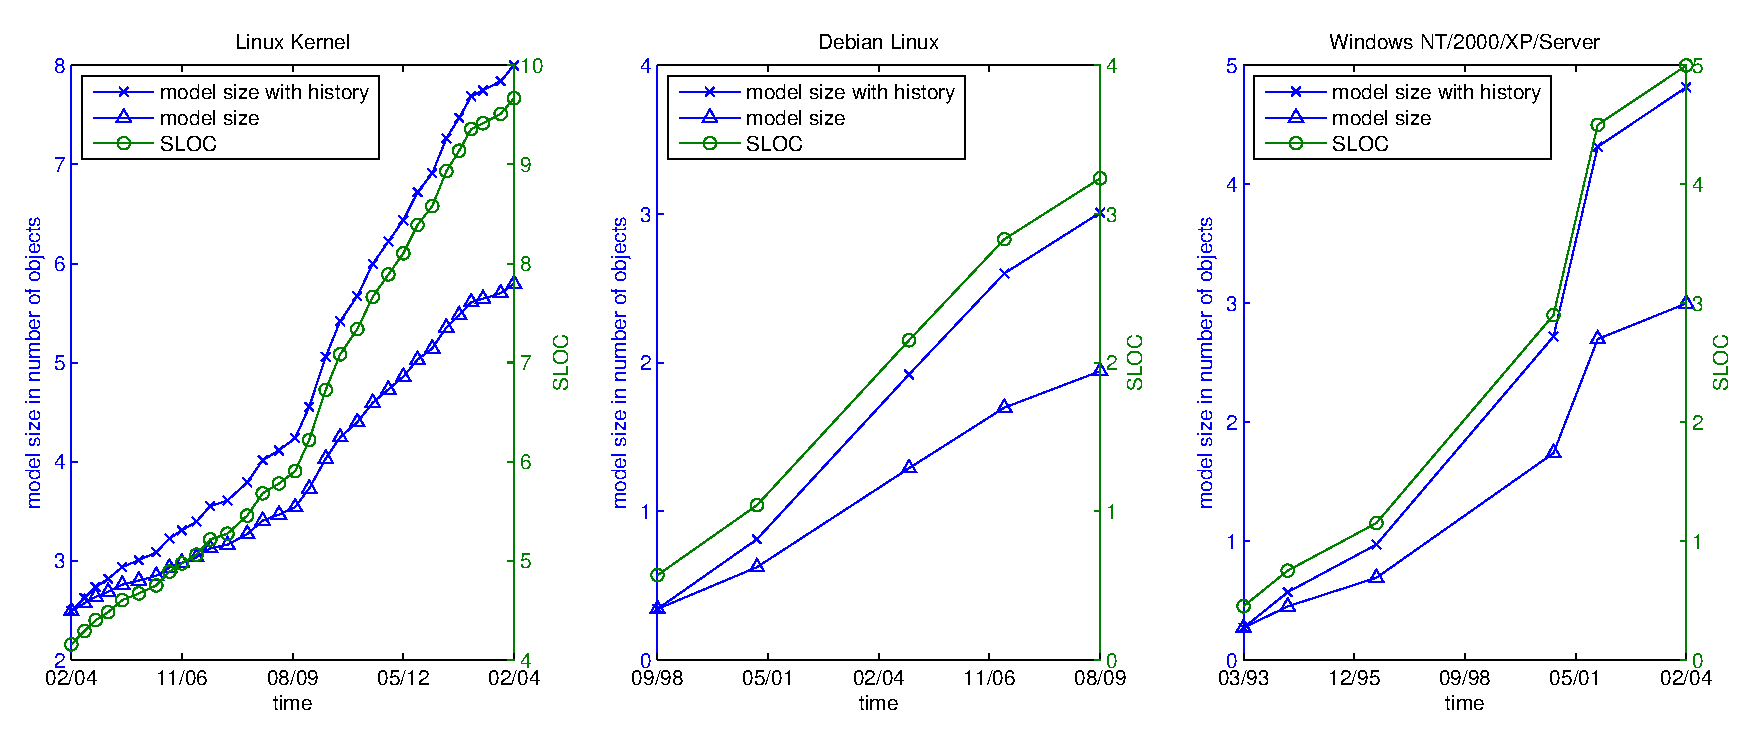
\includegraphics[width=\linewidth]{figures/software_model_sizes}
  \caption{Rough estimates for software code model sizes based on actual SLOC counts for existing software projects.}
  \label{fig:software_model_sizes}
\end{figure}

\tinyparagraph{Usage patterns}
There are two major use cases in today's software development: editing and transforming or compiling. The first use case is either performed on diagrams (graphical editing) or on compilation units (e.g. Java-files, textual editing). Diagram contents roughly corresponds to package contents. Both packages and compilation units are sub-trees within the containment tree of a software model.  Transformations or compilations are usually either done for the whole model or again on a per package or compilation unit basis. Within these aggregates, the (partial) model is traversed. A further use-case is analysis. Analysis is sometimes performed with single queries. But due to performance issues, model analysis is more often performed by traversing the model and by executing multiple queries with techniques similar to model transformations. Software models are only accessed by a few individuals at the same time.

\subsection{Heterogeneous Sensor Data}

Sensor data usually comprises of time series of measured physical values in the environment of a sensor. Our research group build the \emph{Humboldt Wireless Lab}~\cite{hwl}, a 120 node wireless sensor network that produces heterogeneous sensor data: data from a 3 axis accelerometers, data from monitoring all running software components (mostly networking protocols), and other system parameters (e.g. CPU, memory, or radio statistics). We represent and analyze this data with EMF based models (\cite{clickwatch}).

% add cites for SMTL once accepted

\tinyparagraph{Model size}
HWL's network protocols and system software components provide 372 different types of data sets. Each data set is represented as an XML document. Per second each node in the network produces XML entities that translate into an average of 1120 EMF objects. A common experiment with HWL involves 50 nodes and measures of a period of 24\,h. During such an experiment, the network produces a model of $5\times 10^9$ objects. 

\tinyparagraph{Usage patterns}
There are two major use-cases: recording sensor data and analyzing sensor data. Recording sensor data means to store it faster than it is produced. If possible in a manner that supports later analysis. Sensor data is rarely manipulated. Analysis means to access and traverse individual data sets (mostly time series). Each data set or recorded set of data sets is a sub-tree in the sensor data model. Recording and analysis is usually performed by only a single (or a few) individuals at the same time. 

\subsection{Geo-spatial Models}

3D city models are a good example for structured geo-spatial information. The CityGML~\cite{cityGML} standard, provides a set of XML-schemata (building upon other standards, e.g. GML) that function as a meta-model. CityGML models represent the features of a city (boroughs, streets, buildings, floors, rooms, windows, etc.) as a containment hierarchy of objects. Geo spatial models usually come in different levels of details (LOD); CityGML distinguishes 5 LODs, 0-4)~\cite{cityGML}. 

\tinyparagraph{Model size}
As for many cities, a CityGML model is currently established for Berlin~\cite{berlinGML}. The current model of Berlin covers all of Berlin, but mostly on a low-medium level of detail (LOD 1-2). To get an approximation of the model's size, we counted the XML entities. The current Berlin model, contains $128\times 10^6$ objects. Based on numbers and average sizes per feature sizes in the Berlin model, a complete LOD 3-4 model of Berlin would consist of $10^9$ objects. Extrapolating numbers to the world's population that lives in cities, a LOD3-4 \emph{world 3D city model} would contain $10^{12}$.

\tinyparagraph{Usage patterns}
Compared to model manipulation, model access is far more common and its efficient execution is paramount. If accessed, users usually load a containment hierarchies (sub-tree) corresponding to a given set of coordinates or address (geographic location): partial loads. Queries for distinct feature characteristics within a specific geographic location (i.e. with-in such a partial load) are also common. Geo-spatial models are accessed by many people at the same time. 

\subsection*{Summary}

The following table summarizes this section. Two $+$ signs denote that execution times of the respective tasks are vital for the success of the application; a single $+$ denotes that the task is executed often, but performance is not essential; a $-$ denotes that the task is of minor importance.

\begin{center}
\begin{tabular}{|c||c|c|c|c|c|c|}
\hline
\bf{application} & \bf{model size} & \bf{create/mod.} & \bf{traverse} & \bf{query} & \bf{partial load} \\
\hline\hline
software models & $0-10^9$ & + & ++ & + & + \\
\hline
sensor data & $10^9$ & ++ & ++ & - & ++ \\
\hline
geo-spatial models & $10^9-10^{12}$ & - & - & ++ & ++ \\
\hline
\end{tabular}
\end{center}